\chapter{Valutazione dei risultati}\label{ch:evaluation}

  \section{Qualità del codice \& unit testing}
    Durante lo sviluppo, si è cercato di prestare particolare attenzione alla qualità del codice prodotto.

    Si è ritenuto fondamentale, innanzitutto, per favorire la consistenza dello stile, che il codice fosse conforme a uno stile di programmazione riconosciuto.
    Come detto nella~\Cref{subec:quality}, sono stati utilizzati diversi \emph{linter} (ESLint e ktlint)
    per imporre lo stile Airbnb per TypeScript e lo stile ufficiale per Kotlin in tutta la codebase.
    Questo ha permesso di evitare bug comuni riconoscibili attraverso analisi statica
    e potenzialmente permette di rendere il codice, che è pubblico e open-source, maggiormente comprensibile per chi vorrà estenderlo in futuro.

    Inoltre, per garantire il corretto funzionamento delle componenti più cruciali, sono stati creati degli specifici unit test in grado di coprire il codice per quanto possibile.
    L'esecuzione dei test viene effettuata automaticamente da Travis CI su diverse piattaforma ad ogni operazione di push.

    Per quanto riguarda il backend è stato utilizzato JUnit 5 con l'ausilio delle estensioni di Vert.x.
    I report sulla copertura vengono raccolti tramite JaCoCo.

    \unsure[inline]{Quali dettagli dovrei fornire dei test del backend?}

    Anche il frontend è stato testato tramite unit testing.
    In particolare, si è utilizzato la suite Jest per l'esecuzione dei test e la raccolta dei dati di copertura.

    \unsure[inline]{Quali dettagli dovrei fornire dei test del frontend?}

  \section{Valutazione dell'interfaccia}
    Per quanto riguarda la valutazione del client, è stata presa in considerazione principalmente l'esperienza finale dal punto di vista dell'utente web.
    Per avere una misura quantitativa di quanto l'applicazione web si presenti adeguata, si è deciso di utilizzare lo strumento Lighthouse messo a disposizione da Google.

    \emph{Lighthouse} è uno strumento automatizzato open-source, fornito inizialmente con la suite di strumenti \emph{Chrome DevTools}, che permette l'\emph{auditing} di pagine web secondo gli standard premiati dal motore di ricerca di Google.
    Esso verifica
    \begin{inparaitem}
      \item prestazioni di caricamento e navigazione,
      \item accessibilità,
      \item SEO (\emph{\emph{S}earch \emph{E}ngine \emph{O}ptimization}),
      \item buone pratiche di programmazione.
    \end{inparaitem}
    Supporta inoltre controlli aggiuntivi per le PWA (\emph{\emph{P}rogressive \emph{W}eb \emph{A}pp}) se abilitati.

    \begin{figure}
      \centering
      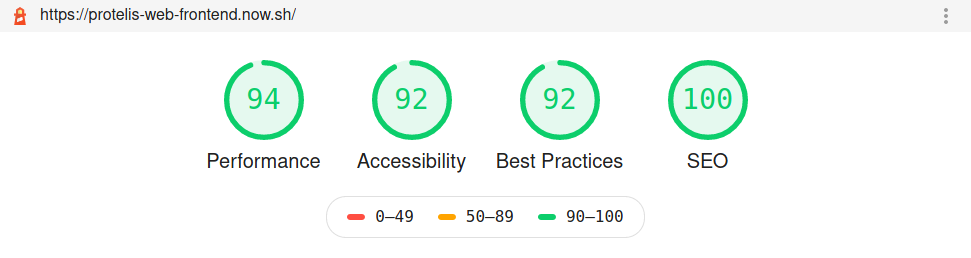
\includegraphics[width=\textwidth]{res/tests/Screenshot_2020-03-04 Lighthouse Report Viewer.png}%
      \caption{Punteggio ottenuto con Google Lighthouse}%
      \label{fig:lighthouse}
    \end{figure}

    Come è possibile vedere in~\Cref{fig:lighthouse}, l'applicazione web ha ottenuto un buon punteggio generale.

    I punteggi di accessibilità e \emph{best practices} sono strettamente legati dalle librerie impiegate, sia in positivo che in negativo:
    il valore elevato deriva da ottimizzazioni della libreria stessa sui componenti che fornisce, cercando di aderire quanto possibile agli standard più moderni;
    le criticità che non portano al 100\% sono legate a limiti difficilmente aggirabili se non configurazioni complesse e fuori tema rispetto all'obiettivo di questa tesi.

    Il punteggio massimo per la SEO, ottenuto ottimizzando la configurazione base generata da React, garantisce, secondo quanto dichiarato da Google, una migliore compatibilità con i motori di ricerca e dunque un ranking migliore.

    Le performance, sulle quali si ha avuto maggiore controllo durante l'implementazione, sono buone, con tempi di primo disegno inferiori al secondo e un ritardo prima di avere possibilità di interazione intorno a \SI{1.6}{\second}.
    A pesare sul punteggio vi è l'assenza di gestione della cache delle richieste, funzionalità non ritenuta importante in questo progetto.

    Volendo ottimizzare, si potrebbe aggiungere il supporto allo standard PWA, secondo le \emph{best practices} documentate da Google.

  \section{Performance}
    % TODO
    \unsure[inline]{Come valuto i risultati? Misure di Performance?}
